\subsection{Partially-commutative polynomial optimization}
\begin{example}
\label{ex:pcpop_hardy}
Consider the problem of certifying genuine multi-partite non-locality in a Bell scenario with n parties where each party performs two dichotomic measurements \cite{PhysRevA.110.L010401}. Here we illustrate the case for two parties. This can be cast as a polynomial optimization problem with variables $X=\{A_1,A_2,B_1,B_2\}$ each being projectors and where $A_i,B_j$ belong to Alice and Bob respectively. The problem reads as follows.
\begin{equation}
   \begin{split}
       p^* &=\underset{\underline{X} , \psi , \mathcal{H}}{inf} \: \braket{\psi, A_1 \mult B_1 \psi}, \\
    & s.t \quad [A_i,B_j] =0, \forall i,j \in \{1,2\}\\
    & s.t \quad A_i^2-A_i = B_j^2-B_j = 0, \forall i,j \in \{1,2\} \\
    & s.t \quad \braket{\psi, A_2 \mult B_1 \psi} = \braket{\psi, A_1 \mult B_2 \psi} = 0, \\
    & s.t \quad \braket{\psi, (1-A_2) \mult (1-B_2) \psi} = 0, \\
    & \qquad \quad \braket{\psi , \psi} = 1. \\ 
\end{split}
\end{equation} 
This can be solved with PCPOP as follows.
\begin{code}
    @pcmonoid M A[2,0] B[2,0]
    Projector.([A;B])
    @comms A B
    build(M)
    obj=A[1]*B[1]
    tr_eq= [[A[2] * B[1],0],[A[1] * B[2],0],[(1-A[2]) * (1-B[2]),0]]
    level=2
    ov,model,var_dict,principal_matrix=npa(obj,level;tr_eq=tr_eq,min=false)
    println("Optimal value is ",ov)
\end{code}
This returns optimal value as $0.0902$ as in \cite{PhysRevA.110.L010401}. The steps to solve a partially-commutative polynomial optimization problem are similar to that of non-commutative polynomial optimization with some differences.
\end{example}
\begin{itemize}
    \item First we define the partially-commutative monoid using the macro \texttt{@pcmonoid}. The first argument is always for the monoid object and the rest for the variables. 
    \item Then, we define which variables commute using the built-in macro \texttt{@comms}. 
    \item Then we define some special operator equality constraints like \emph{projector}, \emph{unitary}, \emph{dichotomic} and \emph{orthogonal pairs} using built-in functions \texttt{Projector,Unitary,Unipotent} and macro \texttt{@ortho} respectively. We leave the general equality constraints to be fed to \texttt{npa} function as the optional argument \texttt{op\_eq}.
    \item Finally, we call the function \texttt{npa} to solve the optimization problem. \texttt{npa} takes the objective polynomial and the level as compulsory arguments and also some optional arguments like arrays of operator inequalities(\texttt{op\_ge}), operator equalities(\texttt{op\_eq}), expectation value equalities(\texttt{tr\_eq}) and inequalities(\texttt{tr\_ge}). The function returns the optimal value, the SDP model, a dictionary that maps the monomial basis to coressponding JuMP variables and finally the principal matrix.
\end{itemize}
\begin{remark}
Notice, that compared to the non-commutative case, where we we enforce all the equality constraint before building the monoid, here we only enforce the special equality constraints like projector, unitary, dichotomic and orthogonality before building the monoid. These special equality constraints are directly and efficiently handled using normal forms and not using Macaulay method which handles the general operator equality constraints. 
\end{remark}
The user interface to define the variables and the monoid is same as in non-commutative case. The macro \texttt{@comms} provides multiple ways to define commutation relations. We illustrate all the options.
\begin{lstlisting}[style=code, mathescape=true]
julia>@pcmonoid M a b # a and b are two hermitian variables
julia>@comms a b #  variable a commutes with variable b
julia>print(a*b,"\n",b*a)
(a)(b)
(a)(b)
julia> a*b==b*a
true
\end{lstlisting}
\begin{lstlisting}[style=code, mathescape=true]
julia> @pcmonoid M A[2,0] B[2,0] # A1,A2 are hermitian variables for Alice and B1,B2 for Bob
julia> @comms A B # all variables of A commute with all variables of B
\end{lstlisting}
\begin{lstlisting}[style=code, mathescape=true]
julia>@pcmonoid M a b c d e f # a,b,c,d,e,f are six hermitian variables
julia>@comms [a,b,c] # to enforce [a,b]=[b,c]=[a,c]=0
julia>a*b*c==c*a*b
true
julia>a*e*b == b*e*a
false 
\end{lstlisting}
To enforce the orthogonality constraint $a*b=0$, we can use the built-in macro \texttt{@ortho} as $\texttt{@ortho a b}$. The \texttt{@ortho} macro works similarly as \texttt{@comms} macro.

For certain equality constraints, the full Gr"obner basis is infinite; even reductions using finite truncations (at a fixed degree) remain costly, and the substitution method in the ncpol2sdpa package~\cite{} is ineffective in that case. We illustrate this with examples of partial commutations whose independence graph have non-transitive orientation[see \cite{} for details] and in which some variables are projectors.  

\begin{example}
  \label{ex:3comms}

    Consider $X=\{a,b,c\}$ where $a,b$ are projectors and $[a,b]=[b,c]=0$. The independence graph is as shown below. 
    \begin{figure}[H]
    \centering
    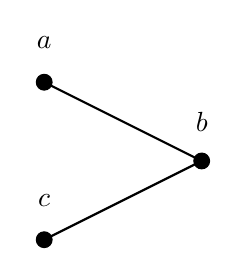
\begin{tikzpicture}[scale=1]
        % w1 label above
        \node at (-5, 2.5) {$a$};
        \node at (-3, 1.5) {$b$};
        \node at (-5, 0.5) {$c$};
        % Draw the vertices
        \filldraw[black] (-5, 2) circle (0.1);
        \filldraw[black] (-3, 1) circle (0.1);
        \filldraw[black] (-5, 0) circle (0.1);
        % Draw the edges
        \draw[thick] (-5, 2) -- (-3, 1);
        \draw[thick] (-3, 1) -- (-5, 0);
    \end{tikzpicture}
    \caption{Independence graph}
    \end{figure}

    We consider the following optimization problem.
\begin{equation}
   \begin{split}
       p^* &=\underset{\underline{X} , \psi , \mathcal{H}}{inf} \: \braket{\psi| \: c\mult a\mult b-b\mult c\mult a\: |\psi}, \\
    & s.t \quad [a,b]=[b,c] =0\\
    & s.t \quad a^2-a = b^2-b = 0 \\
    & \qquad \quad \braket{\psi | \psi} = 1. \\ 
\end{split}
\end{equation} 
With PCPOP, the above problem can be solved as follows.
\begin{code}
    @pcmonoid M a b c
    Projector.([a,b])
    add_comms!([(a,b),(b,c)])
    build(M)
    obj=c*a*b - b*c*a
    level=2
    ov,model,var_dict,principal_matrix=npa(obj,level)
    println("Optimal value is ",ov)
\end{code}
\end{example}

\begin{example}
  \label{ex:4comms}
    Consider $X=\{a,b,c,d\}$ where $a,b$ are projectors and $[a,b]=[b,c]=[c,d]=[a,d]=0$. The independence graph is as shown below. 
    \begin{figure}[H]
    \centering
    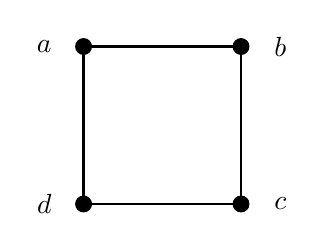
\begin{tikzpicture}[scale=1]
        % w1 label above
        \node at (-5.5, 2) {$a$};
        \node at (-2.5, 2) {$b$};
        \node at (-2.5, 0) {$c$};
        \node at (-5.5, 0) {$d$};
        % Draw the vertices
        \filldraw[black] (-5, 2) circle (0.1);
        \filldraw[black] (-3, 2) circle (0.1);
        \filldraw[black] (-5, 0) circle (0.1);
        \filldraw[black] (-3, 0) circle (0.1);

        % Draw the edges
        \draw[thick] (-5, 2) -- (-3, 2);
        \draw[thick] (-3, 2) -- (-3, 0);
        \draw[thick] (-3, 0) -- (-5, 0);
        \draw[thick] (-5, 0) -- (-5, 2);
    \end{tikzpicture}
    \caption{Independence graph}
    \end{figure}

    We consider the following optimization problem.
\begin{equation}
   \begin{split}
       p^* &=\underset{\underline{X} , \psi , \mathcal{H}}{inf} \: \braket{\psi| \: c\mult d^2\mult b- d^2\mult b\mult c\: |\psi}, \\
    & s.t \quad [a,b]=[b,c]=[c,d]=[a,d]=0\\
    & s.t \quad a^2-a = b^2-b = 0 \\
    & \qquad \quad \braket{\psi | \psi} = 1. \\ 
\end{split}
\end{equation} 
With PCPOP, the above problem can be solved as follows.
\begin{code}
    @pcmonoid M a b c d
    Projector.([a,b])
    add_comms!([(a,b),(b,c),(c,d),(a,d)])
    build(M)
    obj=c*d^2*b - d^2*b*c
    level=2
    ov,model,var_dict,principal_matrix=npa(obj,level)
    println("Optimal value is ",ov)
\end{code}
\end{example}

\begin{example}
\label{ex:5comms}
    Consider $X=\{a,b,c,d,e\}$ where $a,b$ are projectors and $[a,b]=[b,c]=[c,d]=[d,e]=[a,e]=0$. The independence graph is as shown below. 
    \begin{figure}[H]
    \centering
    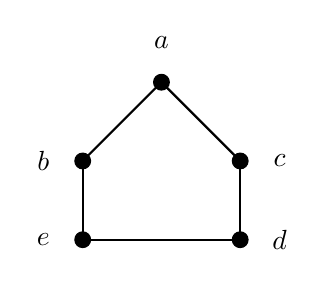
\begin{tikzpicture}[scale=1]
        % w1 label above
        \node at (-4, 3.5) {$a$};
        \node at (-5.5, 2) {$b$};
        \node at (-2.5, 2) {$c$};
        \node at (-2.5, 1) {$d$};
        \node at (-5.5, 1) {$e$};
        % Draw the vertices
        \filldraw[black] (-4, 3) circle (0.1);
        \filldraw[black] (-5, 2) circle (0.1);
        \filldraw[black] (-3, 2) circle (0.1);
        \filldraw[black] (-5, 1) circle (0.1);
        \filldraw[black] (-3, 1) circle (0.1);

        % Draw the edges
        \draw[thick] (-4, 3) -- (-5, 2);
        \draw[thick] (-4, 3) -- (-3, 2);
        \draw[thick] (-3, 2) -- (-3, 1);
        \draw[thick] (-3, 1) -- (-5, 1);
        \draw[thick] (-5, 1) -- (-5, 2);
    \end{tikzpicture}
    \caption{Independence graph}
    \end{figure}

    We consider the following optimization problem.
\begin{equation}
   \begin{split}
       p^* &=\underset{\underline{X} , \psi , \mathcal{H}}{inf} \: \braket{\psi| \: d\mult e^2\mult c- e^2\mult d\mult c\: |\psi}, \\
    & s.t \quad [a,b]=[b,c]=[c,d]=[d,e]=[a,e]=0\\
    & s.t \quad a^2-a = b^2-b = 0 \\
    & \qquad \quad \braket{\psi | \psi} = 1. \\ 
\end{split}
\end{equation} 
With PCPOP, the above problem can be solved as follows.
\begin{code}
    @pcmonoid M a b c d e
    Projector.([a,b])
    add_comms!([(a,b),(b,c),(c,d),(d,e),(a,e)])
    build(M)
    obj=d*e^2*c - e^2*d*c
    level=2
    ov,model,var_dict,principal_matrix=npa(obj,level)
    println("Optimal value is ",ov)
\end{code}
\end{example}